\documentclass[11pt]{dssg}


% \usepackage{fullpage,times,subfigure,fancyhdr}
% % \usepackage{hyperref}
% \usepackage{textcomp}
% \usepackage{verbatim}
% \usepackage{cite}
% \usepackage{times}
\usepackage{amsfonts,amsmath,amssymb,amsthm}
% \usepackage{textcomp}
% \usepackage{url}
% \usepackage{mdwlist}
\usepackage{subfigure}
\usepackage{wrapfig}
\usepackage{sidecap}
% \usepackage{xspace}
\usepackage{algorithm,algorithmic}
% \usepackage[pdftex]{graphicx}
% \usepackage[pdftex]{color}
% % \usepackage[colorlinks=true,pagebackref,linkcolor=magenta]{hyperref}
% \usepackage[sort&compress,colon,square,numbers]{natbib}
% % \usepackage{titlesec}
% \usepackage[breaklinks=true,letterpaper=true,bookmarks=false,]{hyperref}
\usepackage[colorlinks=true,linkcolor=magenta]{hyperref}
\usepackage[sort&compress,colon,square,numbers]{natbib}
% % \usepackage{changepage}
\usepackage{soul}
%\usepackage{denselists}
%\usepackage{scaledfullpage}
\usepackage[dvips]{graphicx}
\usepackage{color}
\usepackage{boxedminipage}
\usepackage{amsfonts}
\usepackage{amsmath}
\usepackage{url}
\usepackage[table]{xcolor}
%\usepackage{times}
%\usepackage{nih}		% PHS 398 Forms
%\usepackage{nihblank}		% For printing on Blank PHS 398 Forms
%\usepackage{confidential}
\usepackage[normalem]{ulem}
\usepackage{comment}
\usepackage{paralist}

\usepackage{chngcntr}


\usepackage{caption}% http://ctan.org/pkg/caption
\usepackage{etoolbox}% http://ctan.org/pkg/etoolbox
\captionsetup{font=small}


% \counterwithin{figure}{section}


\definecolor{MyPlum}{rgb}{0.3,0,0.3}
\definecolor{MyOrange}{rgb}{1,0.5,0}
\definecolor{deep_blue}{rgb}{0,.2,.5}
\definecolor{dark_blue}{rgb}{0,.15,.5}
\usepackage[linecolor=dark_blue, linewidth=1.5pt, skipabove=4pt, nobreak=true]{mdframed}


% 
% \hypersetup{pdftex,  % needed for pdflatex
%   breaklinks=true,  % so long urls are correctly broken across lines
%   colorlinks=true,
%   linkcolor=dark_blue,
%   citecolor=deep_blue,
% }
% 
\usepackage[left,pagewise]{lineno}
\renewcommand{\headrulewidth}{0pt}

% 
% 
\newcommand{\rb}[1]{{\color{red}{\it RB: #1}}}
\newcommand{\ella}[1]{{\color{red}{\it JoVo: #1}}}
\newcommand{\gabi}[1]{{\color{red}{\it gabi: #1}}}
% % \newcommand{\dd}[1]{{\color{MyOrange}{\it Vova: #1}}}
% % \newcommand{\hadoop}{HADOOP}
\newcommand{\db}[1]{{\color{dark_blue}{#1}}}
\newcommand{\bb}[1]{{\textbf{\db{#1}}}}
\newcommand{\ernst}[1]{{\color{red}{\it ernst: #1}}}
\newcommand{\rjv}[1]{{\color{red}{\it RJV: #1}}}
\newcommand{\ray}[1]{{\color{red}{\it ray: #1}}}
\newcommand{\will}[1]{{\color{red}{\it will: #1}}}
\newcommand{\misha}[1]{{\color{red}{\it misha: #1}}}
\newcommand{\guillermo}[1]{{\color{red}{\it guillermo: #1}}}
% 
% \newcommand{\sectn}[1]{\section{#1} \rfoot{\small #1 ~~ \thepage}}
% %\newcommand{\sectn*}[1]{\section*{#1} \rfoot{\small #1 ~~ \thepage}}
% 
% \renewcommand{\thepage}{\thesection-{\arabic{page}}}
\renewcommand{\thesection}{\Roman{section}}   % set the section counter to Alpha
\renewcommand{\thesubsection}{\Roman{section}.\Alph{subsection}}   % set the subsection counter to alpha
% \renewcommand{\thesubsubsection}{\Alph{section}.\arabic{subsection}(\arabic{subsubsection})}   % set the subsection counter to alpha
% 
% 
\makeatletter
% \def\subsize{\@setsize\subsize{8pt}\xipt\@xipt}
 \def\section{\@startsection {section}{1}{\z@}{5pt}{9pt}{\Large\bf\db}}
 \def\subsection{\@startsection {subsection}{2}{\z@}{10pt}{4pt}{\large\bf\db}}
 \def\subsubsection{\@startsection {subsubsection}{2}{\z@}{10pt}{4pt}{\bf\db}}
% \def\subs{\@startsection {subsubsection}{2}{0pt}{5pt}{0pt}{ \subsize\bf\db}}
\def\paragraph{\@startsection {paragraph}{2}{\z@}{10pt}{4pt}{\bf\db}}
% \def\subparagraph{\@startsection {subparagraph}{2}{\z@}{10pt}{4pt}{\qquad \bf\db}}
\newcommand{\para}[1]{\vspace{3pt}\noindent{\bf \db{#1}}}
\newcommand{\subpara}[1]{\vspace{0pt}\qquad{\bf \db{#1.}}}% \newcommand{\paranc}[1]{\vspace{0pt}\noindent{\bf #1}}
% \makeatother
% 
% 
% %% More layout: Get rid of indenting throughout entire document
\setlength{\parindent}{0in}
\setlength{\parskip}{3pt}


% \setlength{\textheight}{10in}
\setlength{\voffset}{0in}
% \setlength{\topmargin}{-15pt}
% 
% \newlength{\saveparindent}
% \setlength{\saveparindent}{\parindent}
% \newlength{\saveparskip}
% \setlength{\saveparskip}{\parskip}
% 
% \newenvironment{newenumerate}{%
% \begin{list}{{\rm \arabic{ctr}.}\hfill}{\usecounter{ctr}\labelwidth=17pt%
% \labelsep=6pt \leftmargin=23pt \topsep=.5pt%
% \setlength{\listparindent}{\saveparindent}%
% \setlength{\parsep}{\saveparskip}%
% \setlength{\itemsep}{5pt} }}{\end{list}}
% 
% \newenvironment{newitemize}{%
% \begin{list}{\hspace{3pt}$\bullet$\hfill}{\labelwidth=12pt%
% \labelsep=3pt \leftmargin=15pt \topsep=1pt%
% \setlength{\listparindent}{\saveparindent}%
% \setlength{\parsep}{\saveparskip}%
% \setlength{\itemsep}{1pt}}}{\end{list}}
% 
% 
% % \pagestyle{fancy}
% % \lhead{}
% % \chead{}
% % \rhead{}
% % \lfoot{}
% % \cfoot{}
% % \rfoot{}
% % \renewcommand{\headrulewidth}{0pt}
% % \renewcommand{\footrulewidth}{0pt}
% 
% \tolerance=1000
% 
% % \setupheads[indentnext=yes]

%%%%%%%%%%%%%%%%%%%%%%%%%%%%%%%%%%%%



%%%%%%% Two column control
\newif\ifdotwocol
\dotwocoltrue   % two col
%\dotwocolfalse   % one col
\long\def\twocol#1#2{\ifdotwocol{#1}\else{#2}\fi}
%%%%%%%

\def\mybeforeequation{\footnotesize}
%\def\mybeforeequation{\small}
%\def\mybeforeequation{}

\def\myafterequation{\renewcommand\baselinestretch{1.1}}
%\def\myafterequation{}

%%%%%%%%%%%%%%%%
%%%%%%%%%%%%%%%%

\def\citeusmark{$^{\textstyle \star}$}
\def\citeus#1#2{\cite{#1}}

\def\crow#1#2{#2}


\def\Paper{grant application}
\def\paper{application}
\def\refappendix{Sec.}

\def\poster{(Poster)}

%Note from brd
\long\def\todo#1{{\bf{To do:}} #1}
%\long\def\todo#1{}
\def\ICRA{IEEE International Conference on Robotics and Automation (ICRA)}

\long\def\squeezable#1{#1}

%\def\a5{$\alpha_{_5}$

\def\a5{5}

%\def\mycaptionsize{\normalsize}
%\def\mycaptionsize{\small}
%\def\mycaptionsize{\small}
\def\mycaptionsize{\footnotesize}
\def\mycodesize{\footnotesize}
\def\myeqnsize{\small}

\def\sheading#1{{\bf #1:}\ }
\def\sheading#1{\subsubsection{#1}}
%\def\sheading#1{\bigskip {\bf #1.}}

\def\ssheading#1{\noindent {\bf #1.}\ } 

\newtheorem{hypothesis}{Hypothesis}
\long\def\hyp#1{\begin{hypothesis} #1 \end{hypothesis}}

\def\cbk#1{[{\em #1}]}

\def\R{\mathbb{R}}
\def\midv{\mathop{\,|\,}}
\def\Fscr{\mathcal{F}}
\def\Gscr{\mathcal{G}}
\def\Sscr{\mathcal{S}}
\def\set#1{{\{#1\}}}
\def\edge{\!\rightarrow\!}
\def\dedge{\!\leftrightarrow\!}
\newcommand{\EOP}{\nolinebreak[1]~~~\hspace*{\fill} $\Box$\vspace*{\parskip}\vspace*{1ex}}
%my way of doing starred references
\newcommand{\mybibitem}[1]{\bibitem{#1} 
\label{mybiblabel:#1}}
\newcommand{\BC}{[}
\newcommand{\EC}{]}
\newcommand{\mycite}[1]{\ref{mybiblabel:#1}\nocite{#1}}
\newcommand{\starcite}[1]{\ref{mybiblabel:#1}\citeusmark\nocite{#1}}


\def\degree{$^\circ$}
\def\R{\mathbb{R}}
\def\Fscr{\mathcal{F}}
\def\set#1{{\{#1\}}}
\def\edge{\!\rightarrow\!}
\def\dedge{\!\leftrightarrow\!}

\long\def\gobble#1{}
\def\Jigsaw{{\sc Jigsaw}}
\def\ahelix{\ensuremath{\alpha}-helix}
\def\ahelices{\ensuremath{\alpha}-helices}
\def\ahelical{$\alpha$-helical}
\def\bstrand{\ensuremath{\beta}-strand}
\def\bstrands{\ensuremath{\beta}-strands}
\def\bsheet{\ensuremath{\beta}-sheet}
\def\bsheets{\ensuremath{\beta}-sheets}
\def\hone{{\ensuremath{^1}\rm{H}}}
\def\htwo{{$^{2}$H}}
\def\cthir{{\ensuremath{^{13}}\rm{C}}}
\def\nfif{{\ensuremath{^{15}}\rm{N}}}
\def\hn{{\rm{H}\ensuremath{^\mathrm{N}}}}
\def\hnone{{\textup{H}\ensuremath{^1_\mathrm{N}}}}
\def\ca{{\rm{C}\ensuremath{^\alpha}}}
\def\catwel{{\ensuremath{^{12}}\rm{C}\ensuremath{^\alpha}}}
\def\ha{{\rm{H}\ensuremath{^\alpha}}}
\def\cb{{\rm{C}\ensuremath{^\beta}}}
\def\hb{{\rm{H}\ensuremath{^\beta}}}
\def\hg{{\rm{H}\ensuremath{^\gamma}}}
\def\dnn{{\ensuremath{d_{\mathrm{NN}}}}}
\def\dan{{\ensuremath{d_{\alpha \mathrm{N}}}}}
\def\jconst{{\ensuremath{^{3}\mathrm{J}_{\mathrm{H}^{\mathrm{N}}\mathrm{H}^{\alpha}}}} }
\def\cbfb{{CBF-$\beta$}}

\newtheorem{defn}{Definition}
\newtheorem{claim}{Claim}

    \gobble{
    \psfrag{CO}[][]{\colorbox{white}{C}}
    \psfrag{OO}[][]{\colorbox{white}{O}}
    \psfrag{CA}[][]{\colorbox{white}{\ca}}
    \psfrag{HA}[][]{\colorbox{white}{\ha}}
    \psfrag{CB}[][]{\colorbox{white}{\cb}}
    \psfrag{HB}[][]{\colorbox{white}{\hb}}
    \psfrag{HN}[][]{\colorbox{white}{\hn}}
    \psfrag{N15}[][]{\colorbox{white}{\nfif}}
    \psfrag{dnn}[][]{\dnn}
    \psfrag{dan}[][]{\dan}
    \psfrag{phi}[][]{$\phi$}
    }

\newenvironment{closeenumerate}{\begin{list}{\arabic{enumi}.}{\topsep=0in\itemsep=0in\parsep=0in\usecounter{enumi}}}{\end{list}}
\def\CR{\hspace{0pt}}           % ``invisible'' space for line break



\newif\ifdbspacing
%\dbspacingtrue  % For double spacing
\dbspacingfalse  % For normal spacing

\ifdbspacing
 \doublespacing
 \newcommand{\capspacing}{\doublespace\mycaptionsize}
\else
 \newcommand{\capspacing}{\mycaptionsize}
\fi

\def\rulefigure{\smallskip\hrule}

% \def\codesize{\normalsize}
\def\codesize{\small}

% Can use macros \be, \ee, \en as shortcuts
%  for \begin{enumerate}, \end{enumerate}, \item
%  respectively.

\def\be{\begin{enumerate}}   % Begin Enumerate
\def\ee{\end{enumerate}}     % End Enumerate
\def\en{\item}               % ENtry (item)
\def\bi{\begin{itemize}}     % Begin Itemize
\def\ei{\end{itemize}}       % End Itemize
\def\bv{\begin{verbatim}}    % Begin Verbatim
\def\ev{\end{verbatim}}      % End Verbatim

\def\matlab{{\sc matlab} }
\def\amber{{\sc amber} }
\def\KS{{$K^*$}}
\def\KSM{{K^*}} % K-Star Math
\def\KSTM{{\tilde{K}^*}}  % K-Star Tilde Math (appx K*)
\def\KOP{{$K^{\dagger}_{o}$}}  % K-Star Optimal partial
\def\KOPM{{K^{\dagger}_{o}}}  % K-Star Optimal partial Math
\def\KP{{$K^{\dagger}$}}  % K-Star partial
\def\KPM{{K^{\dagger}}}  % K-Star partial Math
\def\KTPM{{\tilde{K}^{\dagger}}}  % K-Star Tilde partial Math
\def\KD{{$K_{_D}$}}
\def\KA{{$K_{_A}$}}
\def\qpM{{q_{_P}}}
\def\qlM{{q_{_L}}}
\def\qplM{{q_{_{PL}}}}
\def\qSplM{{q^*_{_{PL}}}}
\def\KSO{{$K^*_{o}$}} % K-Star Optimal
\def\KSOM{{K^*_{o}}}  % K-Star Optimal Math
\def\CBFB{{CBF-$\beta$}}   % Core binding factor beta
% \def\argmin{\mathop{\mathrm{argmin}}}
\def\rhl#1{{\em \underline{RYAN}: *\{{#1}\}*}}
\def\set#1{{\left\{ #1 \right\}}}
\def\Escr{{\mathcal{E}}}
\def\Jscr{{\mathcal{J}}}
\def\Kscr{{\mathcal{K}}}
\def\th{{$^{{\mathrm{th}}}$}}

\newtheorem{proposition}{Proposition}
\newtheorem{lemma}{Lemma}

\setlength{\fboxrule}{1pt}%
\setul{}{1.0pt}

%%%%%%%%%%%%%%%%%%%%%%%%%%%%%%%%%%

\makeatletter
% \renewcommand{\labelitemi}{*}

% \usepackage{helvet}
% \renewcommand{\familydefault}{\sfdefault}

% \newcommand{\jv}{Joshua Vogelstein}
% \newcommand{\jhu}{Johns Hopkins University}
% %\newcommand{\website}{http://jovo.me/}
% \newcommand{\ema}{joshuav@jhu.edu}
% 
% \newcommand{\Vr}{V_{reset}}
% \newcommand{\Vl}{V_{leat}}
% \newcommand{\eqdef}{\overset{\triangle}{=}}
% % \newcommand{\D}[2]{\frac{\partial #1}{\partial #2}}
% \newcommand{\dd}[2]{\frac{\partial ^2 #1}{\partial #2 ^2}}
% \newcommand{\DDD}[3]{\frac{\partial ^2 #1}{\partial #2 \partial #3}}
% \newcommand{\Di}[2]{\frac{\partial ^i #1}{\partial #2 ^i}}
% \newcommand{\grad}{\nabla}
% \newcommand{\Hess}{\nabla\nabla}
% \newcommand{\defn}{\overset{\triangle}{=}}
% 
% \providecommand{\tg}[1]{\textcolor{green}{#1}}
% \providecommand{\tb}[1]{\textcolor{blue}{#1}}
% \providecommand{\tr}[1]{\textcolor{red}{#1}}
% \providecommand{\tk}[1]{\textcolor{black}{#1}}
% \providecommand{\twhite}[1]{\textcolor{white}{#1}}
% \providecommand{\ve}[1]{\boldsymbol{#1}}
% \providecommand{\ma}[1]{\boldsymbol{#1}}
\providecommand{\norm}[1]{\left \lVert#1 \right  \rVert}
% \providecommand{\deter}[1]{\lvert #1 \rvert}
\providecommand{\abs}[1]{\left \lvert #1 \right \rvert}
% \providecommand{\mat}[1]{\left[ #1 \right]}
% \newcommand{\trans}[1]{{#1}^{\ensuremath{\mathsf{T}}}}           % transpose
% \newcommand{\transpose}[1]{{#1}^{\ensuremath{\mathsf{T}}}}           % transpose
\newcommand{\argmax}{\operatornamewithlimits{argmax}}
\newcommand{\argmin}{\operatornamewithlimits{argmin}}
\newcommand{\T}{^{\ensuremath{\mathsf{T}}}}           % transpose
\newcommand{\from}{{\ensuremath{\colon}}}           % :

\newcommand{\Aa}{\mathbb{A}}
\newcommand{\BB}{\mathbb{B}}
\newcommand{\CC}{\mathbb{C}}         
\newcommand{\DD}{\mathbb{D}}         
\newcommand{\EE}{\mathbb{E}}           % expected value
\newcommand{\FF}{\mathbb{F}}         
\newcommand{\GG}{\mathbb{G}}
\newcommand{\HH}{\mathbb{H}}         
\newcommand{\II}{\mathbb{I}}           % indicator function
\newcommand{\LL}{\mathbb{L}}
\newcommand{\MM}{\mathbb{M}}
\newcommand{\NN}{\mathbb{N}}
\newcommand{\PP}{\mathbb{P}}         
\newcommand{\QQ}{\mathbb{Q}}           
\newcommand{\SSS}{\mathbb{S}}           
\newcommand{\VV}{\mathbb{V}}
\newcommand{\XX}{\mathbb{X}}         
\newcommand{\YY}{\mathbb{Y}}
\newcommand{\ZZ}{\mathbb{Z}}         

\newcommand{\iid}{\overset{iid}{\sim}}
\newcommand{\knn}{$k$NN}

% \DeclareMathOperator{\find}{find}

% \newtheorem{thm}{Theorem}
\newcommand{\thma}{\begin{thm}}
\newcommand{\thmb}{\end{thm}}

\newcommand{\mata}{\begin{bmatrix}}
\newcommand{\matb}{\end{bmatrix}}


\newcommand{\bth}{\ve{\theta}}
\newcommand{\hth}{\mh{\theta}}
\newcommand{\htth}{\mh{\theta}}
\newcommand{\bhth}{\mh{\ve{\theta}}}
\newcommand{\thetn}{\ve{\theta}}
\newcommand{\thet}{\thetn}
\newcommand{\theth}{\widehat{\ve{\theta}}}
\newcommand{\theto}{\ve{\theta}'}
\newcommand{\wht}{\widehat{\thet}}
\newcommand{\wtt}{\widetilde{\thet}}
\newcommand{\vth}{\ve{\thet}}
\newcommand{\vTh}{\ve{\Theta}}
\newcommand{\hvth}{\widehat{\ve{\thet}}}
\newcommand{\bTh}{\ve{\Theta}}
\newcommand{\hbth}{\widehat{\thet}}
\newcommand{\tbth}{\tilde{\bth}}

% \newcommand{\p}{P_{\bth}}
\newcommand{\pold}{P_{\bth'}}
\newcommand{\pk}{P_{\widehat{\ve{\theta}}^{(k)}}}
\newcommand{\pT}{P_{\thetn_{Tr}}} %\thetn_T
\newcommand{\pO}{P_{\thetn_o}} %\thetn_o
% \newcommand{\Q}{Q(\thetn,\theto)}
% \newcommand{\m}{m^{\ast}}
% \newcommand{\q}{q(\ve{H}_t)}
\newcommand{\Ca}{[\text{Ca}^{2+}]}

\newcommand{\Lik}{\mathcal{L}}
\newcommand{\Cae}{[\widehat{\text{Ca}}^{2+}]}
\newcommand{\Cav}{\ve{C}}%[\ve{\text{Ca}}^{2+}]}
\newcommand{\sml}{\sqrt{\ma{\lambda}}}
\newcommand{\ml}{\ma{\lambda}}
\newcommand{\nw}{\widehat{n}}
\newcommand{\nv}{\vec{n}}
\newcommand{\Ae}{\widehat{A}}
\newcommand{\te}{\widehat{\tau}}
\newcommand{\maxn}{\max_{\ve{n}: n_t \geq 0}}
% \newcommand{\V}{\text{Var}}

\providecommand{\ms}[1]{\mathsf{#1}}
\providecommand{\mc}[1]{\mathcal{#1}}
\providecommand{\mb}[1]{\boldsymbol{#1}}
\providecommand{\mbb}[1]{\mathbb{#1}}
\providecommand{\mv}[1]{\vec{#1}}
\providecommand{\mh}[1]{\hat{#1}}
\providecommand{\wh}[1]{\widehat{#1}}
\providecommand{\mhv}[1]{\mh{\mv{#1}}}
\providecommand{\mvh}[1]{\mv{\mh{#1}}}
\providecommand{\mt}[1]{\widetilde{#1}}
\providecommand{\mhc}[1]{\hat{\mathcal{#1}}}
\providecommand{\mbc}[1]{\mb{\mathcal{#1}}}
\providecommand{\mvc}[1]{\mv{\mathcal{#1}}}
\providecommand{\mtc}[1]{\widetilde{\mathcal{#1}}}
\providecommand{\mth}[1]{\mt{\mh{#1}}}
\providecommand{\mht}[1]{\mh{\mt{#1}}}
\providecommand{\mhb}[1]{\hat{\boldsymbol{#1}}}
\providecommand{\whb}[1]{\widehat{\boldsymbol{#1}}}
\providecommand{\mvb}[1]{\vec{\boldsymbol{#1}}}
\providecommand{\mtb}[1]{\widetilde{\boldsymbol{#1}}}

\newcommand{\PmcP}{P \in \mc{P}}
\newcommand{\mP}{\mathbb{P}}

\newcommand{\del}{\delta}
\newcommand{\sig}{\sigma}
\newcommand{\lam}{\lambda}
\newcommand{\gam}{\gamma}
\newcommand{\eps}{\varepsilon}

\newcommand{\Del}{\Delta}
\newcommand{\Sig}{\Sigma}
\newcommand{\Lam}{\Lambda}
\newcommand{\Gam}{\Gamma}

\newcommand{\dvs}{\dot{\bs}_t}
\newcommand{\dvw}{\dot{\bw}_t}
\newcommand{\dvx}{\dot{\bx}_t}
\newcommand{\dvy}{\dot{\by}_t}

\newcommand{\ft}{f_{\ve{\thet}}}
\newcommand{\gt}{g_{\ve{\thet}}}
\newcommand{\hht}{h_{\thetn}}

\newcommand{\Real}{\mathbb{R}}

\newcommand{\wconv}{\overset{i.p.}{\rightarrow}}
\newcommand{\sconv}{\overset{i.p.}{\rightarrow}}
\newcommand{\conv}{\rightarrow}
\newcommand{\pconv}{\overset{p}{\conv}}
\newcommand{\mcE}{\mathcal{E}}
\newcommand{\mcT}{\mathcal{T}}
\newcommand{\mcG}{\mathcal{G}}
\newcommand{\mcM}{\mathcal{M}}
\newcommand{\mcL}{\mathcal{L}}
\newcommand{\hatmcE}{\widehat{\mcE}}
\newcommand{\hatp}{\widehat{p}}
\newcommand{\hatP}{\widehat{P}}
\newcommand{\hatQ}{\widehat{Q}}
\newcommand{\hatL}{\widehat{L}}
\newcommand{\mhP}{\widehat{\PP}}
\newcommand{\tildeA}{\widetilde{A}}

\newcommand{\defa}{\begin{defi}}
\newcommand{\defb}{\end{defi}}
\newcommand{\defeq}{\overset{\triangle}{=}}


% \newcommand{\ss}{\mc{S}}
% \newcommand{\mhc}{\mh{\mc{S}}_n}

% \newcommand{\Real}{\mathbb{R}}
% \newcommand{\bTh}{\mb{\Theta}}
% \newcommand{\ra}{\rightarrow}
% \newcommand{\la}{\leftarrow}
\newcommand{\bX}{\mb{X}}

% \newcommand{\bv}{\mb{v}}
% \newcommand{\ba}{\mb{a}}
% \newcommand{\bd}{\mb{d}}
% \newcommand{\balpha}{\mb{\alpha}}
% \newcommand{\conv}{\rightarrow}  
% \newcommand{\xx}{\langle \bx_u^\la, \bx_v^\ra\rangle}  
% \DeclareMathOperator*{\argmax}{arg \hspace{1pt} max \hspace{2pt}}
% \DeclareMathOperator*{\argmin}{arg \hspace{1pt} min \hspace{2pt}}
% \newcommand{\norm}[1]{\left \lVert#1 \right  \rVert}
% 


% \newcommand{\theHalgorithm}{\arabic{algorithm}}


\DeclareMathOperator{\Delti}{\mathbf{\Delta}^{-1}}
\DeclareMathOperator{\Delt}{Q} %\mathbf{\Delta}}
% \DeclareMathOperator{\Gam}{\mathbf{\Gamma}}
\DeclareMathOperator{\Gami}{\mathbf{\Gamma}^{-1}}
\DeclareMathOperator{\Sigb}{\mathbf{\Sigma}}
\DeclareMathOperator{\Ri}{\mathbf{\R}^{-1}}
\DeclareMathOperator{\A}{A}
\DeclareMathOperator{\W}{\mathbf{W}}
\DeclareMathOperator{\V}{\mathbf{V}}
\DeclareMathOperator{\U}{\mathbf{U}}
\DeclareMathOperator{\C}{\mathbf{C}}
\DeclareMathOperator{\uvec}{\mathbf{u}}
\DeclareMathOperator{\D}{\mathbf{D}}
\DeclareMathOperator{\Q}{\mathbf{Q}}
% \DeclareMathOperator{\R}{R} %\mathbf{P}}
\DeclareMathOperator{\Y}{\mathbf{Y}}
\DeclareMathOperator{\B}{\mathbf{B}}
\DeclareMathOperator{\Hmat}{\mathbf{H}}
\DeclareMathOperator{\Gmat}{\mathbf{G}}
\DeclareMathOperator{\X}{\mathbf{X}}
\DeclareMathOperator{\Cmat}{C} %\mathbf{L}}
\DeclareMathOperator{\Pmat}{\mathbf{P}}
\DeclareMathOperator{\veta}{\mathbf{\mb{v}}}
\DeclareMathOperator*{\minimize}{\mathrm{minimize}}
\DeclareMathOperator*{\maximize}{\mathrm{maximize}}
\DeclareMathOperator*{\Ymod}{\mathbf{\Y}}
\DeclareMathOperator*{\Bmod}{\mathbf{B}}
\DeclareMathOperator*{\Hmod}{\mathbf{H}}
\DeclareMathOperator*{\Lmod}{\mathbf{L}}
\DeclareMathOperator*{\Xmod}{\mathbf{\X}}
% \DeclareMathOperator*{\mb{v}mod}{\mathbf{\mb{v}}}

\newcommand{\elegans}{\emph{C. elegans} }

\newcommand{\FAQ}{\texttt{FAQ} }

\providecommand{\tg}[1]{\textcolor{green}{#1}}
\providecommand{\tb}[1]{\textcolor{blue}{#1}}
\providecommand{\tr}[1]{\textcolor{red}{#1}}

\newcommand{\Qs}{Q}
\newcommand{\mcS}{\mc{S}}
\newcommand{\mcU}{\mc{U}}

\newcommand{\mbd}{\mb{d}}
\newcommand{\mbD}{\mb{D}}
\newcommand{\mbx}{\mb{x}}
\newcommand{\mbX}{\mb{X}}
\newcommand{\mby}{\mb{y}}
\newcommand{\mbY}{\mb{Y}}

\newcommand{\mtbd}{\mtb{d}}
\newcommand{\mtbD}{\mtb{D}}
\newcommand{\mtbx}{\mtb{x}}
\newcommand{\mtbX}{\mtb{X}}
\newcommand{\mtby}{\mtb{y}}
\newcommand{\mtbY}{\mtb{Y}}

% \floatname{algorithm}{Procedure}
% \renewcommand{\algorithmicrequire}{\textbf{Input:}}
% \renewcommand{\algorithmicensure}{\textbf{Output:}}
% \floatname{algorithm}{Pseudocode}

\providecommand{\sct}[1]{{\sc \texttt{#1}}}

\newcommand{\aimDa}{{\sc \bb{Aim D.1: Deploy Data-Intensive Computing Ecosystem for Storage, Dissemination, and Analysis of Big Neuroscience Data.}}}
\newcommand{\aimDb}{{\sc \bb{Aim D.2: Convert Massive Raw 2D Monochromatic Images from Multiple Resolutions and Modalities to 3D Multispectral Co-Registered Volumes.}}}
\newcommand{\aimDc}{{\sc \bb{Aim D.3: Create Neural Semantic Scenes from Multispectral Volumes.}}}
\newcommand{\aimDd}{{\sc \bb{Aim D.4: Transform Neural Semantic Scenes to Knowledge via Statistical Analysis, Models, and Implementations at Scale.}}}


% \setlength{\abovedisplayskip}{-5pt}
% \setlength{\belowdisplayskip}{-15pt}
% \setlength{\abovedisplayshortskip}{-15pt}
% \setlength{\belowdisplayshortskip}{-5pt}
% \baselineskip=0pt
% \abovedisplayskip=0.7cm
% \abovedisplayshortskip=-0.3cm
% \belowdisplayskip=0.7cm
% \belowdisplayshortskip=0.4cm
% % \setlength{\voffset}{-15pt}
% % \setlength{\headsep}{15pt}
% % \setlength{\textheight}{9.5in}
% \setlength{\belowcaptionskip}{0pt}

\setlength{\textheight}{10in}
\setlength{\textwidth}{6.5in}
% \setlength{\leftmargin}{15pt}
% \setlength{\rightmargin}{1in}
\setlength{\oddsidemargin}{0in}
% \setlength{\evensidemargin}{1in}

% \pagenumbering{arabic}
\setlength{\tabcolsep}{1pt}

% \linenumbers


\tolerance=500

\begin{document}

\title{Humans in Autonomy: Verifiable, Multi-Scale, Co-Design}

\author{Ella Atkins, Randal Burns, and Mark Campbell}

\maketitle




\section*{Motivation and Key Research Questions}

The evolution of autonomy has revealed that the humans need to be inextricably involved in all dimensions of autonomous systems, not 
just managing those systems, but seamlessly integrating human capabilities, human information gathering, and human decision making.
\begin{center}
\parbox[c]{6in}{
{\em ``$\ldots$ the true value of unmanned systems is not to provide a direct human replacement, but rather to extend and complement human capability.''} \\
\hspace*{20pt} DSB Task Force Report, The Role of Autonomy in DoD Systems, 2012.
}
\end{center}
The DSB asserts that the benefits of Autonomy lie in unlimited persistence, reducing risk to humans, and reducing cognitive load.
Autonomy should in no way eliminate or reduces human capabilities.  This lead to shift in thinking in which autonomy is a capability to
be integrated into a complex human-machine system,  rather than a functional replacement for a human.

With this conceptual shift, the question arises: How can autonomy integrate into human-machine systems so that they maximize the 
performance the system as a whole?  Insight into system performance requires measures and models of human performance 
both standalone and in the presence of autonomy and the capability to understand the systems that are multi-scale, complex
networks of humans and autonomy.

Beyond performance, as autonomy grows in complexity, scope, and scale, guarantees that autonomous systems 
operate correctly and within bounds according
\begin{center}
\parbox[c]{6in}{
{\em ``Autonomous and semi-autonomous weapon systems shall be designed to allow 
commanders and operators to exercise appropriate levels of human judgment over the use of force.''}
\hspace*{20pt} A. B. Carter, DoD Directive 3000.09, November 21, 2012
}
\end{center}



%Ensure that autonomy doesn’t compromise our humanity
%\begin{center}
%\parbox[c]{6in}{
%{\em ``To comply with international humanitarian law, fully autonomous weapons would need human qualities that they inherently lack.''} \\
%\hspace*{20pt} Human Rights Watch, “Losing Humanity”, November 19, 2012
%%}
%\end{center}

\subsection*{Definition of Autonomy}
(DoD Autonomy Priority Steering Council, Nov 2012)
Definition of Autonomy: “capability and freedom to self-direct to achieve mission objectives”

“Military Power in the 21st Century will be defined by our ability to adapt – this is THE hallmark of autonomy”

Key Technical Challenge Areas/Gaps
Human-Autonomy Interaction and Collaboration
Scalability
Machine Intelligence
Verification and Validation

\subsection*{Key Research Questions:}

How do we model, verify, and utilize humans as collaborative decision makers and actors in correct-by-construct autonomous systems?

How do we create multi-scale, model-based autonomy (controllers, communication, and computation) that scales to the battlespace?

How do we co-design complex mission systems to optimally and acceptably incorporate human and autonomy decision-makers and actors?










\section*{Background}

The conclusions and implications of this think piece are built upon five key technical areas: Verification \& Validation, which is common in computer software and autonomy; correct by construction controllers which are generated with guarantees; probabilistic modeling of human decision making; collaborative autonomy, and model based system engineering. Each of these are briefly described here, with a few example references. 

\subsection*{Verification \& Validation (software v. autonomy)}

A recent study by the Office of the US Air Force Chief Scientist~\cite{tech-horizons2011} cited Verification and Validation (V\&V) is a key limitation in the ability to achieve the high impact gains that can be realized from autonomy. 
\begin{center}
\parbox[c]{6in}{
{\em ``Increased use of autonomy$\ldots$  will depend on development of entirely new methods for enabling `trust in autonomy' through verification and validation (V\&V) of the near-infinite state systems that result from high levels of adaptability and autonomy.''} \\
\hspace*{20pt} A Vision for Air Force Science and Technology 2010-30, USAF Chief Scientist, 2011.
}
\end{center}

It is important to first understand the definitions of Verification and Validation:
\begin{center}
\parbox[c]{6in}{
{\em Verification: Requirements evaluation {\em during} development} \\[0.1 in]
{\em Validation: Requirements evaluation {\em after} integration} %\\
%\hspace*{20pt} A Vision for Air Force Science and Technology 2010-30, USAF Chief Scientist, 2011.
}
\end{center}
Thus, the process of verification is to incrementally and systematically evaluate whether a system or subsystem is meeting requirements during the design process. Validation, on the other hand, evaluates whether the completed system meets the end customer requirements in a practical setting. If done well, Verification can speed up of the Validation process because portions of the underlying system have already been verified. 

The process of V\&V has been known for a long time, and is a formal part of nearly any systems engineering process~\cite{Blanchard2010}. The importance  of systematic processes has increased as the complexity/safety/security of the system has increased, such as in cars, airplanes, and spacecraft. V\&V for these systems has typically taken the form of empirical testing because it is closer to the end operational state, and people typically accept empirical testing easier than other options such as simulations. 

Most of these complex systems have grown in complexity more because of software growth than other components. Autonomous systems are particular challenging, as the physical system has not changed as much as the internal `intelligence' of the software. With the software growth, however, comes the typical challenges in verification of the system (now, a physical+software system). Dr.\ Werner Dahm, former Chief Scientist of the Air Force, has given several talks on the Air Force study in Ref.~\cite{tech-horizons2011}, and cited the growth and errors in software. A small summary is given below:

\begin{table}
\begin{center}
\begin{tabular}{l|c}
System &  Lines of Code (loc)\\ \hline
F-4A & 1,000\\
F-15A &  50,000\\
F-16C &  300,000\\
F-22 &  2,500,000\\
F-35 &  18,000,000
\end{tabular}
\caption{Critical lines of code for aircraft; $\sim$4-6 errors per 1000 LOC, $\sim$0.1-1.0 errors per 1000 critical LOC}
   \label{table:loc}
\end{center}
\end{table}

Current V\&V methods are not sustainable as systems increase in complexity, given this growth. Dr.\ Dahm argues that current systems with autonomous elements are tested to exhaustion of the budget, rather than to a formal level of V\&V. 

V\&V in software has also increased in importance over the years with the growth of programs and applications.  Risk management for large software systems has
lead to the ``spiral model'' of development \cite{boehm1988spiral} that builds out systems based on successive cycles each that incorporate V\&V and links V\&V to 
design and the evaluation of risk.  The process commonly employs multiple groups for V\&V that are independent from developers, including a test team that are 
part of the software development process and users and customers that participate in user acceptance {\em beta} testing.  

With all applications, the time required for the processes for V\&V increases, creating pressures on safety/security/costs, etc. As such, recent research in the software engineering community has focused on developing automated, and formal, verification tools. Formal methods is a well established area of research concerned with formally specifying systems and properties, developing techniques to prove/disprove that a system satisfies a property (verification), and in some cases, developing methods to generate a system from required properties (synthesis). Model checking~\cite{clarke_99} is a verification technique that exhaustively searches the state space of a system in order to either verify that a property holds over all of the system's executions or to find a counter example, e.g.\  using temporal logic of actions \cite{tla}.  Formal V\&V tools have matured so that they can provide formal proofs for large concurrent systems; the Alloy Analyzer has been used to correct the Chord peer-to-peer protocol \cite{alloychord} and verify the Internet's Border Gateway Protocol \cite{alloybgp}. Other advances adds V\&V capabilities to existing languages and development tools, such as the verifiable C compiler \cite{vcc}.  


%Model checking has been extremely successful~\cite{Var06b,ClarkeMcmillan90,pentiumMC} and many industrial and academic model checkers have been developed (e.g.~\citen{spin,NuSmv,IBM_MC}). 


The robotics community has borrowed/expanded these concepts for the verification of autonomy. In particular, research has been conducted in developing approaches for formal verification of software for autonomous systems. Spin~\cite{spin} and NuSVM~\cite{nusvm} are two examples of powerful model checkers that have been used to verify autonomy software generated from higher level specifications. SAT solvers (e.g.~\cite{een03minisat,Herbstritt01zchaff:modifications}) are powerful tools that check whether a propositional logic formula has a satisfying assignment, a technique that exhaustively searches all executions of a system up to length $k$. All of these tools typically check logical consistency of a specification and reports on deadlocks, race conditions, incompleteness, and  assumptions. 

%Over the past several years, robotics researchers have developed methods for automatically synthesizing complex, hybrid controllers from high-level task specifications in a manner that provides guarantees about the behavior of the robot (e.g.~\cite{mishra_95,SavvasCDC04,QBIZicra04,FKGPicra_05,FKGPcdc_05,BBEFKP06,belta_06,KGFPicra_07,CKGiros_07,KGC_ram08,KB_TAC08,F_aut,
%frazzoli_acc08,KGFP_TRO09,Karaman2009,Bhatia2010,Wongpiromsarn2010,Wongpiromsarn2011}). 


Most recently, the community has developed `probabilistic model checkers' such as PRISM \cite{Kwiatkowska2001,prism} which are designed to verify software to a particular level of probability. These tools typically verify a system through symbolic data structures and algorithms as well as exhaustive search. Importantly, state of the art tools are being used to verify software and autonomy, even probabilistically.

\subsection*{Correct by construction controllers}

In the application of robotics, the formal verification methods have been used to generate `correct by construction' controllers from high-level task specifications in a manner that provides guarantees about the behavior of the autonomy~\cite{mishra_95,FKGPcdc_05,kress2009temporal,Wongpiromsarn2011}. This is the process whereby a system is modeled and a list of specifications in generated. The specifications are typically at the higher level, such as `visit all rooms until you find my keys' or 'do not go into room X.' In this case, hybrid controllers (discrete and continuous elements) are automatically generated and guaranteed to satisfy the original specifications listed. If the specifications cannot be met, then the controller is not generated. The flow chart of the process is given below. 

\begin{figure}[h] 
\centering
   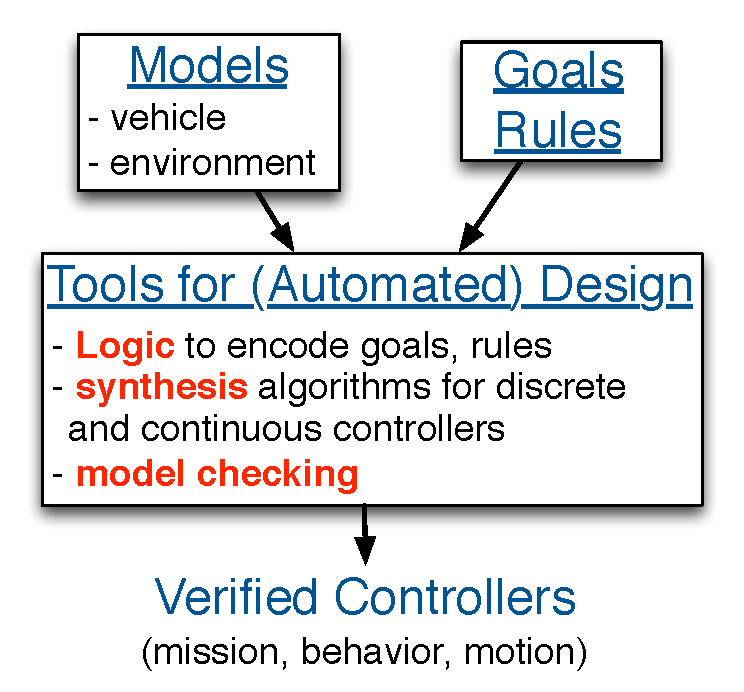
\includegraphics[width=2.5in]{correct-by-construction.pdf} 
   \caption{correct by construction example}
   \label{fig:correct-by-construction}
\end{figure}

These concepts have been extended to using probabilistic model checkers, and this work is most applicable to the concepts proposed in this think piece. Typically, an off-the-shelf model checking software such as PRISM~\cite{Kwiatkowska2001,prism} is used to find the probabilities of satisfying the desired set of logic based specifications. Given a full characterization of the system (known probabilities for environment and sensor models), model checking techniques can be used to find upper and lower bounds on the probability that the autonomy will satisfy the set of specifications.

Figure~\ref{fig:taxi-taxi} shows a recent example of a taxi driver with a specification on collision probability~\cite{johnson2012execution}. In this case, the authors have defined collision probability based on the current location density of an object (e.g.\ another car) in an environment, a map of the road structure, and a temporal/probabilistic prediction of the location density into the future, based on typical driving standards (Figure~\ref{fig:taxi-taxi}(left)). A collision bound is then calculated and used as a design specification for the controller. A controller can then be generated by selecting a `desired probability of collision', and generating and  checking a controller for the taxi driving in an environment with other cars. Figure~\ref{fig:taxi-taxi}(right) shows the case when the other cars in the environment are modeled as not obeying any rules of the road.By selecting a `desired probability of collision' and generating a controller, different autonomous driving behaviors can be realized, such as conservative driving or agressive driving. 


\begin{figure}[h] 
\centering
   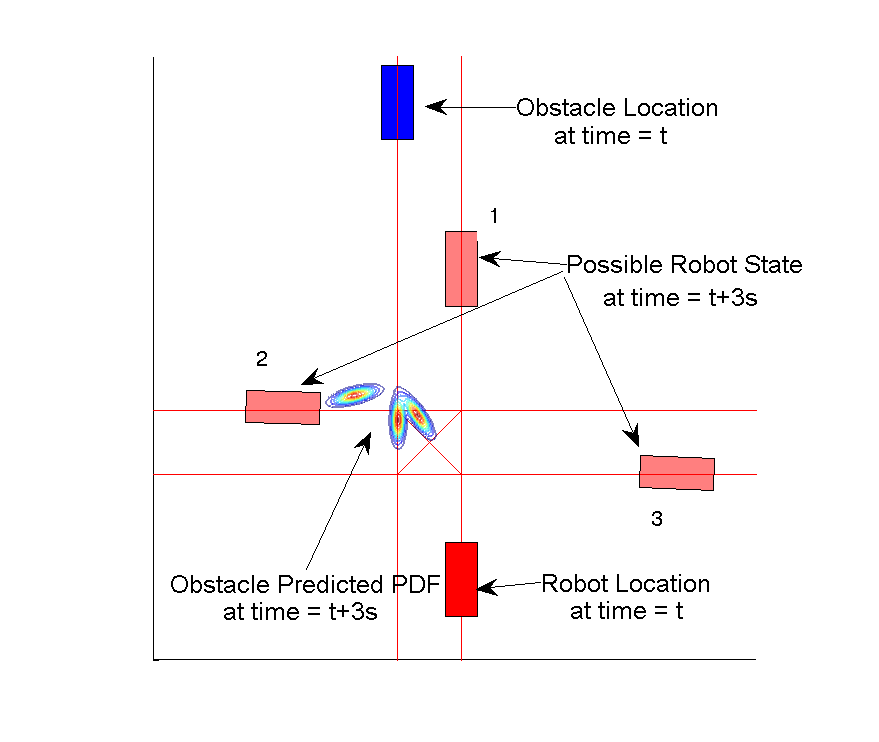
\includegraphics[width=3.0in]{coll_prob_inst.pdf} 
  % \label{fig:collision}
   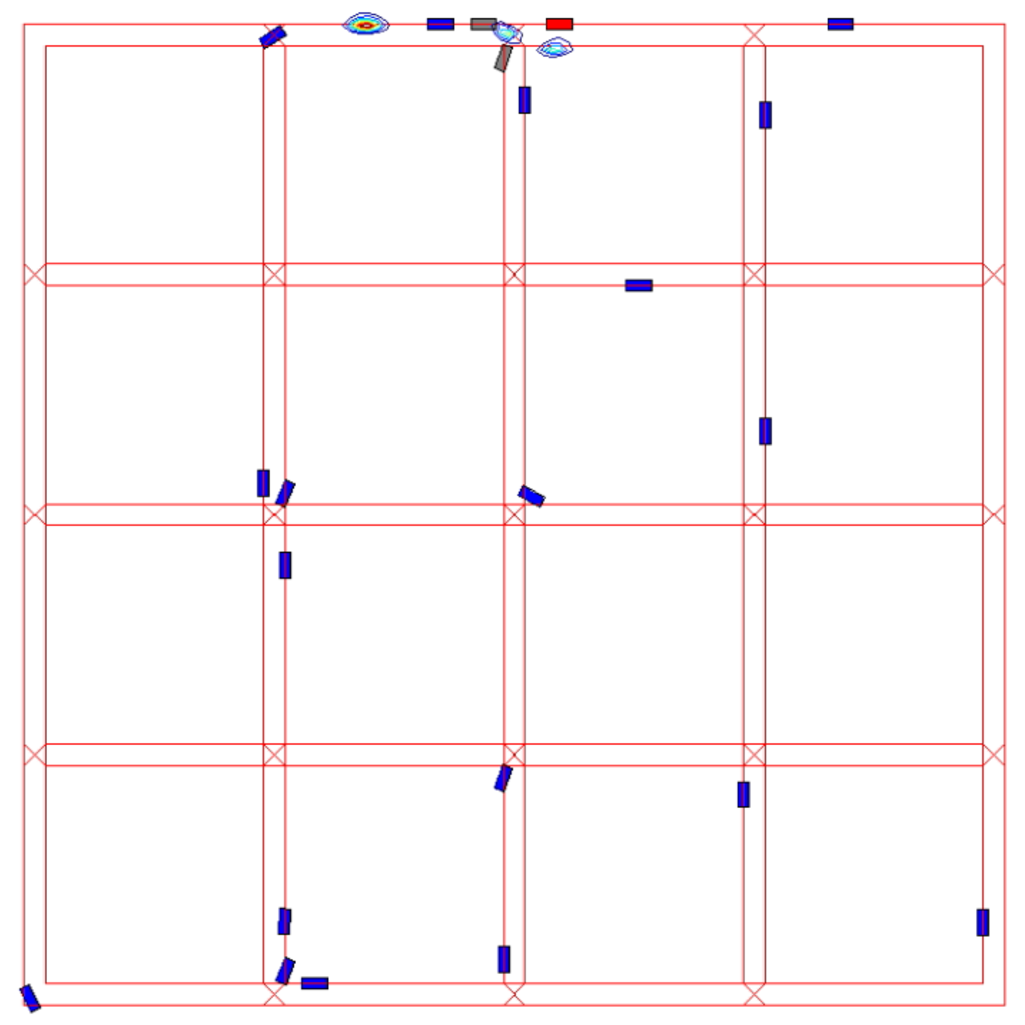
\includegraphics[width=2.5in]{taxi-driver.pdf} 
   \caption{collision probability taxi driver example}
   \label{fig:taxi-taxi}
\end{figure}

Given that there are now approaches to generating software for autonomous systems that are probabilistically correct, can we now begin to include human interaction (and models of humans) such that the controllers are designed with humans in mind?

\subsection*{Probabilistic modeling and humans}

Modeling even a portion of human capabilities will enable the ability to plan and optimize an integrated human-autonomy system. Modeling human-machine interactions in large-scale networked systems can be useful in making research more prospective, rather than reactive, which has typically been the characteristic of previous research on humans and automation. Modeling can also inform the design of future interfaces to support operators of multiple UV systems in the presence of concurrent operational and cognitive uncertainties. 

Research in modeling of human capabilities has been on-going to many years, from the early work on simple cognitive functions and interaction with autonomy~\cite{Sheridan92}, to more recent work attempting to model extensive cognitive capabilities~\cite{anderson1997act} and even the brain~\cite{brain2013}. Integrated databases have been developed for modeling/prediction of perception and motor skills~\cite{epic,Kieras99a,Byrne03a,actrpm}. Currently, these databases are focused on low level human skills, and do not integrate with the environment (such as the use of autonomy models). ACT-R~\cite{anderson1997act} is a cognitive architecture attempting to model a full range of human cognitive tasks, including the way we perceive, think about, and act on the world. The ACT-R architecture has developed modules  representing perceptual attention, motor programming, long-term declarative memory, goal processing, mental imagery and procedural competence. Applications have included air traffic control~\cite{lebiere2001multi,taatgen2006modeling} and multiple agents in military environments~\cite{best2006cognitive}. 


The human factors community, on the other hand, has focused on empirically driven tests in order to gain insightful observation of trends, but not formal models; one fruitful area has been in supervisory control of UAVs where several human operators are typically required to control current unmanned aerial vehicle (UAV) platforms~\cite{cooke2006human,cummings2007operator}.  Given the goal of one operator to many UAVs, automation support, even if imperfect, is mandated~\cite{barnes2010human,parasuraman2005flexible,parasuraman2009adaptive}. However, the extra task load generated by handling imperfect automation may interfere with adequately supervising a larger number of UAVs. Recent estimates of an operator's capacity to control multiple UAVs range from 1 to 16~\cite{Wickens2006},  
 but more precise estimates may be calculated by considering the impact of UAV coordination demands, UAV interaction and neglect times, automation reliability, mission type and operator tasks and the task-to-robot ratio~\cite{Wickens2006,cummings2008predicting,de2011adaptive,galster2006managing,parasuraman1997humans}. Research on operators in Air Traffic Control~\cite{Galster01a,Rantanen04a} has provided valuable insight into how users make decisions as a function of parameters such as stress, interface type, and time. 
These works typically derive key performance metrics from trends in the data, but do not formally model them. 

Many generic `non-cognitive' probabilistic models have been proposed as alternatives to well-known detailed cognitive computational models for predicting human-in-the-loop performance in networked unmanned vehicle applications. In \cite{Fan10} and \cite{Heger06}, for instance, human operators are modeled dynamically via probabilistic Markov models in order to capture random transitions between abstract discrete states that influence decision-making and task performance metrics. In \cite{Donmez10}, discrete-event task simulations with probability distributions on operator servicing times are used to explicitly model the performance effects of changing workload and vehicle utilization in a multi-UAV supervisory task. Both cognitive and non-cognitive dynamic probabilistic human-operator models can be used to generate sample-based performance prediction statistics via repeated random simulations of closed-loop task execution, and as such can provide useful insight into specific scenarios that lead to good/bad operator performance. However, such dynamic probabilistic models require a high level of detail and much training data to explicitly account for the effects of various task/network-related factors (e.g.\ number of agents, task load). These models also do not explicitly account for individual factors, e.g.\ differences in working memory capacity. Furthermore, many simulations must be run with dynamic models in order to make performance predictions for a single set of operating conditions, which can be cumbersome for exploring many different network/task conditions. 

A new class of probabilistic models has recently been developed that are potentially useful for prediction and verification of human operator performance in human-autonomysystems, either in the sense of performing detailed analyses related to dynamical process simulations or performing gross `high-level' analyses of human-machine system performance that abstract away certain dynamical details. Two of these models, \emph{Gaussian Process (GP) regression} and \emph{Bayesian networks (BN)}, can enable direct `function-like' performance  predictions without requiring simulations or an explicit model of the operator's decision-making processes \cite{Ergo}. Any expected variability arising from differences in these and other unmodeled factors related to task dynamics are described by the estimated probabilities associated with each prediction. A third type of model,  \emph{probabilistic discriminative classification models}, can be used to capture stochastic \emph{non-Markovian state-dependent switching behaviors} for discrete supervisory decision making by human operators in detailed process models \cite{Bourgault2007}, \cite{Ahmed2008}, \cite{Ahmed2011a}, which is currently not realizable with the probabilistic Markov or discrete event models mentioned above. 

As an example, consider the case of probabilistically modeling human observations at a macro level (human observations and/or tasks), in an effort to more formally exchange information with an autonomous system. Both discrete~\cite{Ahmed2012a} and continuous human inputs~\cite{Bourgault2008} have been modeled, including a rich set of structured inputs such as  `The target is near the tree and heading quickly toward you' or `There is nothing behind the wall.'  The key challenge is probabilistically modeling terms such as `near' or `behind'. 

Leveraging the fact that discrete random variables nicely represent soft (human) categorical information, the human information has been shown to be well-modeled via probabilistic classifiers  \cite{Ahmed-TRO-2012, Ahmed-ICRA-2010, Ahmed-ACC-2011a,Ahmed10SigPro}.  These classifiers are typically learned from human observation data, such as computer point and click; chat inputs; and natural language processing. Figure~\ref{fig:likelihood} shows a simple example of learning soft human categorical information from data.

\begin{figure}[h] 
\centering
   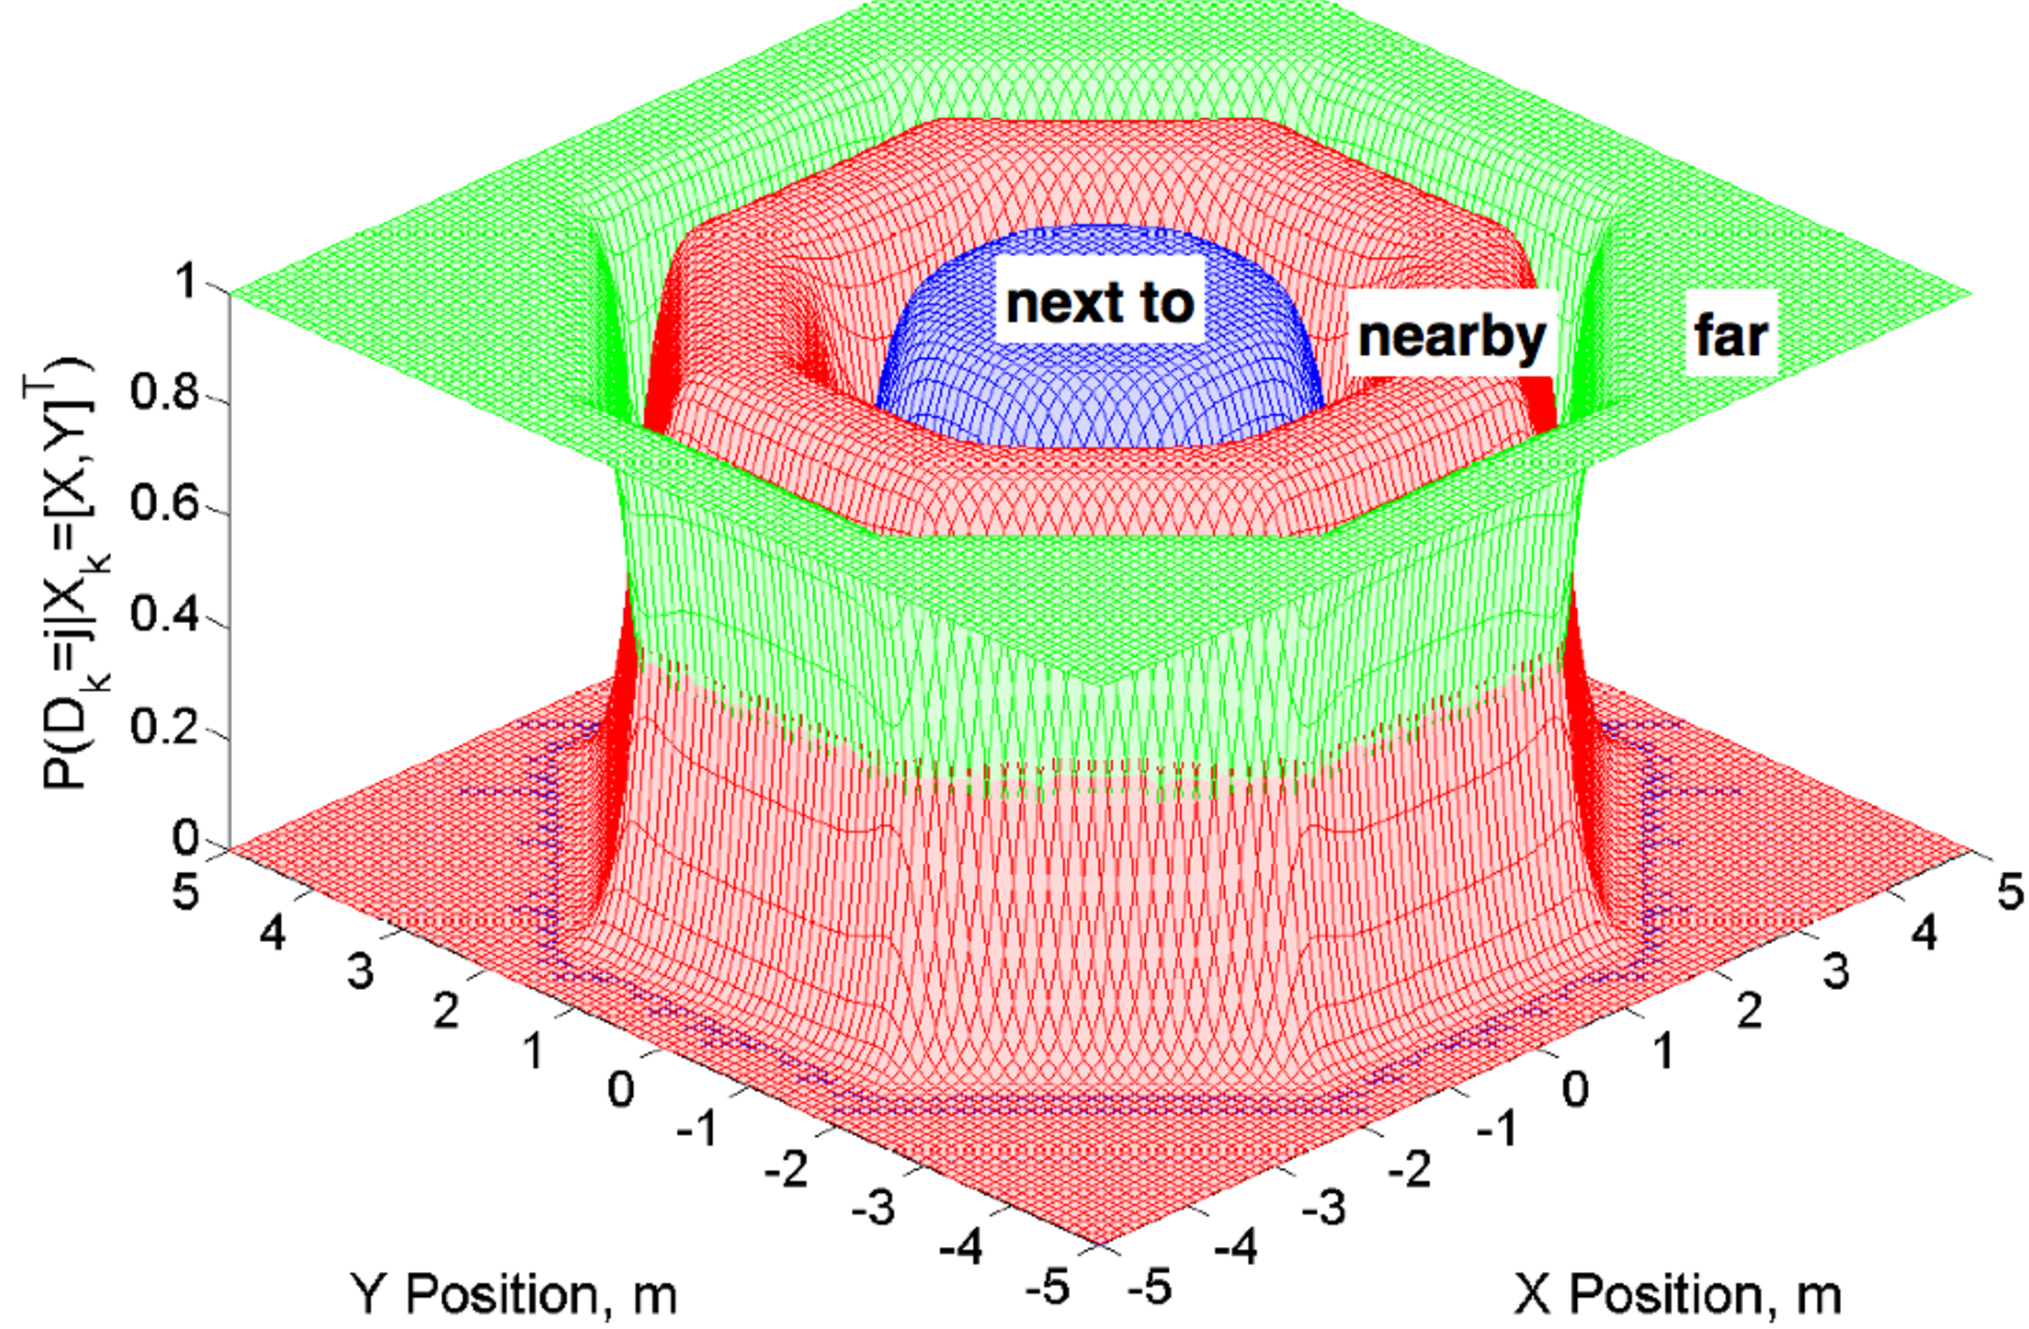
\includegraphics[width=3.5in]{mms.pdf} 
   \caption{Learned likelihood model for relations `next to', `nearby', and `far.' }
   \label{fig:likelihood}
\end{figure}

These likelihood functions then enable a host of subsequent functions, from cooperative planning to information fusion and inference. Ref.~\cite{Ahmed10SigPro} empirically investigates how human information can be used by an autonomous robot in a search mission. Even though  human subjects could not directly command robots, it was found that fusing human and robot observations greatly improved object search performance (i.e.\ number of targets found, time to find objects, object localization error) compared with baseline searches using robot observations alone. Human observations were particularly useful for correcting missed object detections and reducing the distances traveled by the robot, whereas the use of \textit{negative information} (e.g., `Nothing is near the bridge') was shown to be particularly important in the integrated human+robot team performance.

The use of Gaussian Process models has been shown to be particularly insightful into human tasking, including variations over users. In a collaboration between researchers in the human factors community and the autonomy community, collected operator data was modeled using different statistical modeling methods to study the ability to predict human operator performance in an  air defense simulation scenario~\cite{Ahmed2013a}; performance metrics were modeled as a function of task load, message quality, and operator working memory capacity. It was found that state-of-the-art Gaussian Process (GP) regression models can make predictions with uncertainty bounds that are more informative than traditional linear regression and discrete Bayesian network (BN) prediction models. More specifically, off-line tests of human operator metrics (such as working memory) are predictive in eventual performance of the operators in the UAV tasking environment (such as red zone performance). The GP models also nicely capture uncertainty in area of the model with little date, and trends/anomalies with user capabilities. Figure~\ref{fig:prob-humans} shows an example of one such predictive model, where task performance is captured as a function of working memory, which can be evaluated off-line in a priori tests. Several studies have shown that individual differences in working memory capacity play a major role in determining how well a person can focus attention on visual tasks and cope with distractors such as irrelevant messages~\cite{Engle02}. More generally, working memory is thought to be a key component of executive control processes that underlie effective multi-tasking and decision-making in time-critical tasks~\cite{Parasuraman2010,Endsley95}. Therefore, individual differences in working memory capacity could be modeled and used in developing verifiable specifications. 

\begin{figure}[h] 
   \centering
   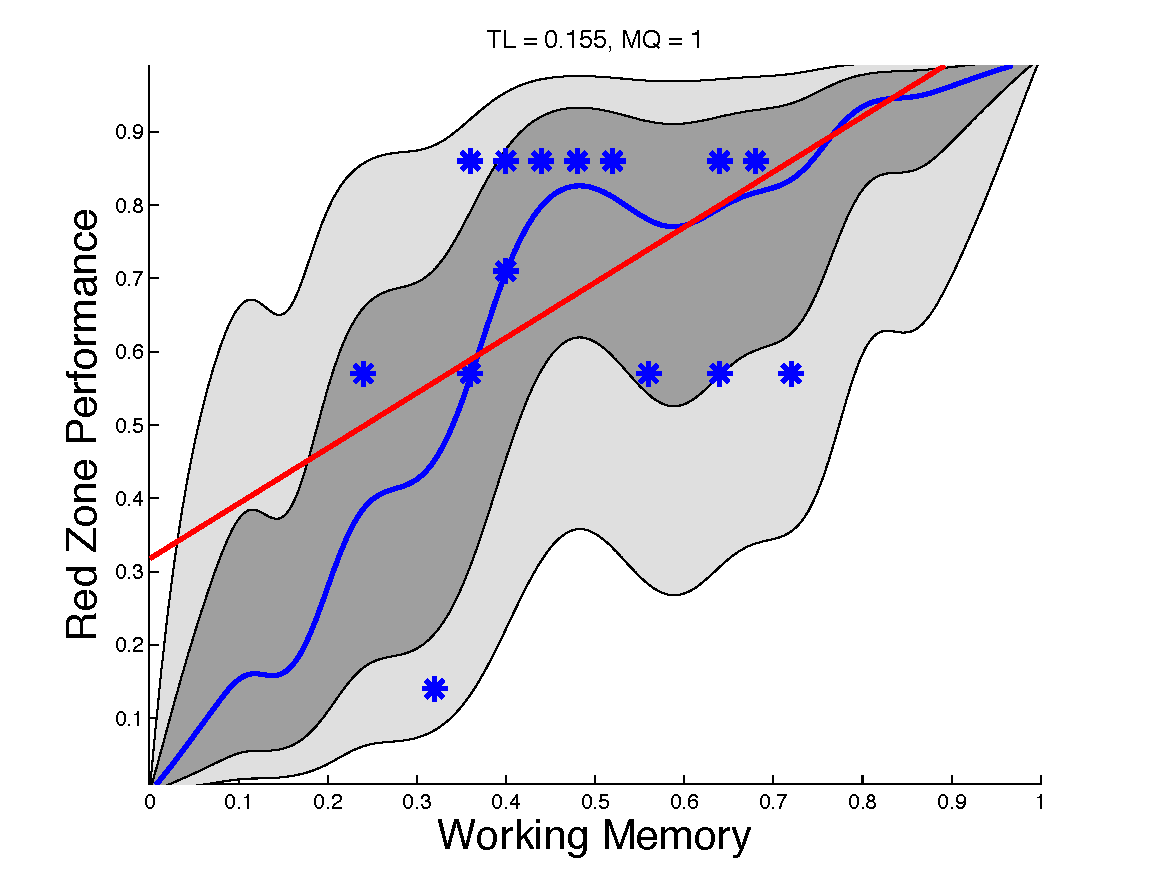
\includegraphics[width=3.5in]{GP-fig.pdf} 
   \caption{Example of probabilistic modeling of human capabilities, correlating performance with working memory.}
   \label{fig:prob-humans}
\end{figure}

In summary, there are many classes of models of human tasking, behaviors, and decision making. Importantly, there is a growing maturity in probabilistic models of human decision making can could enable fundamental studies in formal verification of human-autonomy systems. 


\subsection*{Collaborative autonomy}

\mc{TODO write this section.  Then revised by Ella.}

Collaboration over computation, communication, navigation, and sensing

Multi-vehicle collaboration 
Decentralized task selection / allocation (Market protocols - Wellman et al, Optimization - How et al) 
Cooperative path planning (Tsourdos et al)
Scalability through swarm-based techniques (e.g., consensus, potential field)  (McLain et al)

Collaborative human-autonomy systems
Human intent prediction (e.g. partially-observable Markov Decision Process) (Karami et al)
Adaptive tasking (Parasuram et al)
Use metrics (e.g., confidence) to decide when to ask for help (Fong et al) 
Apply perspective-taking to project companion awareness state (Trafton et al)


Capable strategies for collaborative autonomy systems exist and can be 
leveraged for co-design of human-autonomy systems


\subsection*{Model-based system engineering}

\ella{TODO}

Transition from functional decomposition..
Does not scale well
Difficult to verify


…to Model-based System Engineering 
State-based models of each actor are generated.
Each model is re-used over all phases of system engineering
Improves scalability and consistency
State analysis offers a formal method to verify behaviors
Successfully applied to single-actor systems (e.g., spacecraft missions)





%Reference Mission - do we want this?
%
%Mission
%Identify thermal signatures/people of interest
%Detect and avoid or disable IEDs
%Pervasive human and autonomy elements
%High-altitude UAV 
%Large-area monitoring, long-range communications
%Visual/hyperspectral imagery
%Remote operators and analysts
%Group of small UAVs

%Thermal field imaging and video
%Local operators and analysts
%Ground robots:  IED detect and disarm
%Humans deploy and operate locally
%Intelligence collection and dissemination
%Humans:  direct observation; hand-carried devices (e.g., cell phones)
%Manned vehicles (onboard sensors/ computers/comms)
%Remote analysts/data centers


\section*{Key Research Directions}

%Identify capability gaps and define research objectives that integrate autonomy and humans (as command, analysts, operators, and soldiers) that are:
%Model-based, probabilistic, and verifiable (correct by construction)
%Scalable: self-organizing networks of heterogeneous actors that perform navigation, sensing, communication, and computation
%Agile: can be rapidly validated and deployed for specific exploitation missions
%

Given the motivation from the DSB and other DoD studies, and the background in these five areas, our goal was to identify capability gaps and key research objectives that integrate autonomy and humans (as command, analysts, operators, and soldiers) that are:\vspace*{-0.1 in}
\begin{itemize}
\item Model-based, probabilistic, and verifiable (correct by construction)\vspace*{-0.1 in}
\item Scalable: self-organizing networks of heterogeneous actors that perform navigation, sensing, communication, and computation\vspace*{-0.1 in}
\item Agile: can be rapidly validated and deployed for specific exploitation missions\vspace*{-0.1 in}
\end{itemize}

Research directions are described below that will enable these goals. 

\subsection*{Probabilistic Models of Human Capabilities in Correct by Construction Frameworks}

A key research direction is to leverage probabilistic models of human capabilities, and integrate these models into formal frameworks that enable the generation of correct by construction controllers for autonomous systems. Importantly, not all human capabilities have to be modeled; only {\it some} capabilities. And, these models can be probabilistic because the current state of the art in formal methods includes formal tools that consider probability. 

These models can be derived from underlying knowledge of human capabilities, but will mostly be derived from data collected from human tests. Models could be general (a group of humans), or custom (a specific person). A key challenge is minimizing the data collection required to develop such models.  As models of human capabilities mature, they can be integrated into the same framework, and new controllers will be automatically generated that are richer in their ability to work together with humans. 

If a framework exists whereby probabilistic models of human capabilities are integrated into a verifiable framework, then we could:
\vspace*{-0.1 in}
\begin{itemize}
\item Automatically verify (and auto-generate) correct by construction controllers for autonomy. These controllers would be designed with the {\it integrated} human+autonomous system in mind because the specifications are on the task itself, and the models include both the humans and autonomy.  \vspace*{-0.1 in}
\item Generate autonomy software that is `matched' to human capabilities. Given that a different probabilistic model of human capabilities could be developed for different people, it is envisioned that the associated controllers that are automatically generated will consider each person individually. \vspace*{-0.1 in}
\item Speed validation. In any V\&V framework, any improvement in verification (such as increasing speed with automatic verification of formal methods), will in turn speed the end validation process.  \vspace*{-0.1 in}
\end{itemize}

As an example, consider the case of a network of humans and autonomous robots working together on a task, such as surveillance of an area, rescue mission in a forest or building, or other. Figure~\ref{fig:collaboration} shows an abstraction of such a network, with $N$ autonomous vehicles. For this example, we will assume that the human analyzes data feeds for objects and false detections. During a prior testing, models of human capabilities of three particular operators showed that they each have important characteristics:\vspace*{-0.1 in}
\begin{itemize}
\item Operator A has faster eye-hand coordination\vspace*{-0.1 in}
\item Operator B has a photographic memory\vspace*{-0.1 in}
\item Operator C's performance drops rapidly with task load\vspace*{-0.1 in}
\end{itemize}

Given models of these capabilities, the concept of {\it `personalized autonomy'} can be realized whereby the correct-by-construction controller for the autonomous takes these abilities into account. Importantly, the controller is designed with {\it collaborative performance} for the task in mind, not separately. This capability would be useful not only for the original design effort, but also operational deployment with the concept of adaptive tasking~\cite{parasuraman2009adaptive}.

\begin{figure}[h] %  figure placement: here, top, bottom, or page
   \centering
   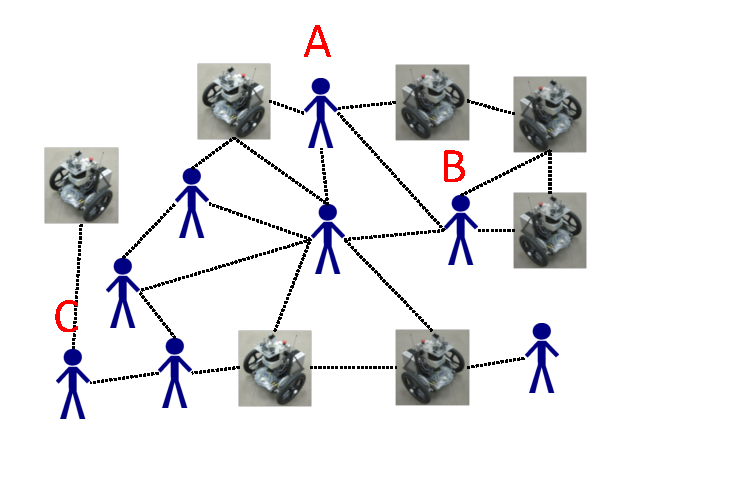
\includegraphics[height=1.5in]{collaboration.pdf} 
   \caption{A network of humans and autonomous systems working together on a task.}
   \label{fig:collaboration}
\end{figure}



\subsection*{Rapid Validation}

A key challenge in future systems is the speed and ability to validate systems prior to deployment. Future autonomy (adaptive, agile) are near infinite state systems, and traditional empirical validation (Test \& Evaluate, T\&E) will not scale~\cite{tech-horizons2011}. 

An example from the DARPA Urban Challenge (DUC) in 2007 crystallized these challenges~\cite{Campbell2010e,Miller2008}. The Cornell team developed an autonomous driving car for the competition. In the 12-18 months prior to the competition, the Cornell team tested and evaluated sub-components and the integrated system, with much of the final six months devoted to systems level testing and evaluation (i.e.\ validation). During the semi-finals of the DUC, Cornell's car, Skynet, could not navigate through a course with many cars parked in either side of the road; this was because the road was narrow, and Skynet is large (a Chevrolet Tahoe). The only way to navigate the course was enable Skynet to slightly cross over the double yellow line in the middle of the road - a capability that the Cornell team took great lengths to avoid. 

In order to make it into the DUC finals, the Cornell team had to make a small software change (a few lines of code) in order to enable Skynet to navigate closer to side cars and over the double yellow line. However, the Cornell team kept asking the same questions: {\it Will this change create other problems? Will this change invalidate the months of validation tests that the team had completed}. In the end, Skynet completed both the semi-finals and finals, completing the competition as one of six finishers. However, not without a lot of stress about not knowing the effects of such a small change. 

One `promise' of a verifiable, probabilistic, correct by construction framework is a shorter validation time. We envision that such tools will enable this improvement. Consider the case of a single operator and UAV, working together on a surveillance task (Figure~\ref{fig:uav-operator}). The specific task is to find and identify certain people in crowded spaces. The operator and UAV must work together on such a task, as the UAV must position itself appropriately (height, location); search and maintain camera field of view on important people; continue to fly why completing its sensing task. The human tasks the UAV to a general area, watches the video, and picks the object of interest that the UAV must track. Consider that the UAV, software, and operator interface were developed, and validation tests occurred over many months that demonstrated reliability to a high level of probability. 

Here is an important question: {\it After one year in operation, the DoD wants to add a new capability, that of automatic entity detection in the UAV software, and use this detection to re-task the UAV.}  Will the past T\&E validation be invalidated? i.e.\ not useful any more? Or can some be used? How much additional T\&E is required to deploy the system again? 

Further, acceptance should be based on the completed task (search, ID, track objects on the ground), and this task is dependent on {\it both} the human and UAV. Thus, if the UAV performs better at its tasks, but the human does not understand/trust the new software, the {\it integrated} human+UAV system could perform worse than it did previously. 

%Example:
%Sensory UAV
%Deployed after FULL test and evaluation (T\&E)
%After a year in operation, would like to add new capability:
%Automatic entity detection for re-tasking
%Past: Need T\&E again?
%Future: Auto-generation of correct by construction (verified) software

\begin{figure}[h] %  figure placement: here, top, bottom, or page
   \centering
   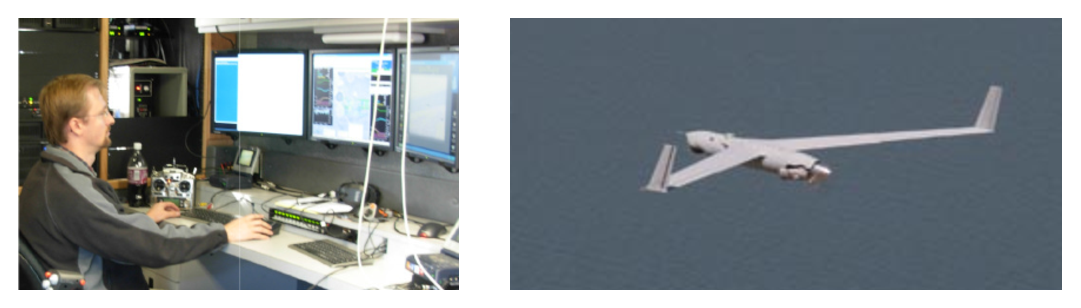
\includegraphics[height=1.5in]{uav-operator.pdf} 
   \caption{An operator tasking a UAV. }
   \label{fig:uav-operator}
\end{figure}

%MC try to Merge with the example. (one slide)
%Takeaway is for a general or Arthi
%Cite Dahm smally
%from SOA and correctness
%Yellow line / car example (?)

While the proposed framework may not solve all problems, it is conceivable that if the software for the UAV was auto-generated to create probabilistically correct by construction (verified) software, then it is conceivable that the addition of UAV capabilities (and perhaps some human tests/models) would enable a faster verification process. 



\subsection*{Multi-scale architectures for human autonomy}

\rb{TODO}
% - I took this out temporarily to send to Bob then put the placeholder back in.  -Ella

\subsection*{Human-Automation System Co-Design}

% \ella{TODO}
Model-based systems engineering holds promise to improve scalability and reusability in complex 
engineered systems but to-date has only been used to design automation and autonomy system elements.
In traditional systems engineering processes, humans are primarily considered through interfaces 
specified in the design, not as integral elements of the system being designed.  
There is good reason 
for this trend:  while a hardware and software system element can be fully customized, the human 
cannot and should not be ``customized'' in the sense of being genetically altered or reconstructed.
However, human capabilities are versatile and can be observed/modeled.  A human actor can then 
be trained to effectively assume a particular role in a collaborative human-automation system, 
and this human training can itself be optimized as part of the overall system design.

We propose the study of human-automation system {\em co-design} in which the systems engineering 
effort models and optimizes the holistic system over human-machine system trade spaces.~\footnote{This 
process of making design choices over a complex systems trade space including humans and automation 
is cited as one of the three primary views for making decisions in ``The Role of Autonomy in DoD 
Systems'' (Defense Science Board, July 2012).}  For a truly integrated co-design process, 
appropriate models, metrics, design space variables, and constraints must be defined across
both human and autonomy elements of the system.  Designs should be free to assign each role to
human actors, autonomous actors, or a team of both based on defined models and metrics.  

A number of challenging research issues must be addressed before co-design can be effective.
Open questions include:
\begin{itemize}
\item How do we model the roles and capabilities of the human?
\item How do we allocate human and autonomy elements during the design process?
\item How do we define common metrics for the human and autonomy elements?
\end{itemize}

The outcome of the co-design systems engineering process will be a product that requires
human and autonomy actors to prepare and deploy effectively over a long term.  The system
lifecycle will involve designing then executing missions, learning from results, 
and adapting the system and actors to improve future mission effectiveness.  The implementation
of a co-designed subsystem will look quite different depending on whether the role assigned to
that subsystem is accomplished by a human or autonomy actor.  The basic question to be addressed for each is:

\begin{itemize}
\item {\em Human:} What training and profiling and profiling will best enable accurate 
model development and mission readiness?
\item {\em Autonomy:} What software and hardware development, database preparation, 
and verification activities will optimize capabilities?
\item {\em Both:} How will human-autonomy actors (subsystems) interact, and over what time
scales can mission design and adaptation be performed?
\end{itemize}

Consider the person of interest and IED detection reference mission proposed above and
shown previously in Figure~\ref{fig:ref-mission}.  This mission contains some capabilities that are
unique to humans and autonomy actors and others that are candidates for co-design.
Humans are uniquely able to directly interact with the local population, and humans will
be assigned responsibility for weapon handling and discharge.  Airborne sensors will almost 
certainly be carried by unmanned aircraft, and autonomy will be responsible for high-speed 
data manipulation and communication.  On the other hand, data-to-decisions activities may be 
assumed by humans, autonomy, or a collaboration of both.  Human and autonomy actors are both
capable of collecting and disseminating data as well as mobilizing assets. 

Human-autonomy interactions are required at the mission level (wide-area) and in the immediate
area of the operation.  Wide-area collaborations will center around big data analysis 
and interpretation, while local-area collaborations will strive to achieve shared 
and sufficiently comprehensive situational awareness.  Local-area collaborations will also need to offer 
effective support for soldiers particularly in life-threatening, fast-paced situations. 
Collaboration between wide-area and local-area system elements is crucial and will involve
direct communication (voice/text) from human actors in combination with data streams from 
autonomy and collaborative system elements.  While the co-designed collaborative human-autonomy 
system will be unquestionably 
``complex'', achieving an effective co-design process holds substantial promise for improving
future mission effectiveness.



\section*{Implications: Potential Impact}

%From slides:
%
%New complex missions mandate new human-autonomy collaboration
%
%Technical advancements in our three topics will:
%Further the DSB goal of seamless, natural, and efficient collaboration of humans and autonomy
%Robustly deploy human-autonomy at the mission scale (not the subsystem scale)
%Model and design human and autonomy elements into an optimized collaborative system
%
%From slide notes:
%
%Goal:  Pursue fundamental research that contributes to bridging the human-autonomy gap
%Furthers the DSB goal of ?seamless, natural, and efficient collaboration of humans and autonomy.?
%??
%Multi-scale:  Robustly deploy human-autonomy at the mission scale (not the subsystem scale)
%Co-Design:  Model and design human and autonomy elements into an optimized collaborative system
%
%Want to make human elements effective?
%Include restatement of DSB human-autonomy goals.
%Human-autonomy collaboration (not interaction).
%Seamless, natural, and efficient collaboration of humans and autonomy.


%Concrete gaps from steering committee
%Specific research directions to address human-autonomy systems
%
%This is where we stay away from our Nos
%  acquistition
%  policy law treaty
% trust and deployment
%  security

%From last discussion slide, see also Galen's notes:
%
%Our initial tack was to make inroads into acceptance.  It was hard.  Why?
%How far can modeling of human capabilities go? 
%Can we formalize trust?
%Can acceptance be accomplished without full system validation?
%How will real and perceived risk change?

%Galen's notes:
%
%?	Q. Are humans on an equal footing to material constructs? In a model. A. Model a human as an autonomous component. Model the human capability and action. Q2. Then you assume that your models are accurate? A2. Yes, this is a challenge we need to do.
%?	Q. Is it probabilistically correct for each object or all the objects together?
%?	Q. Do google cars use this? 
%?	Q. Do you have an idea of what point of errors in the code would be unsustainable? What is the break point. F35C is 25M lines of code. A. The tightness of integration impacts the vulnerability. More modularity in the codes; and in verification and validation of it.
%?	Q. Is trust just an issue of risk? A. No it is more complicated than that.
%?	Q. Given that integration challenges are formidable, what is the role of formal methods in validating the software? A. Modular approach. Q2. About trust? A2. You can formalize correctness, but then how does this translate to trust? Formalisms are powerful at scale. If we could model trust, could integrate it into the formalism. 
%?	Q. Now software comes from many places in the world. Did you consider the issues with this problem? What if there is a rouge partner with software that verifies correctly, i.e. appears to be correct, but in fact has bad intent? A. Address in system engineering ? as a part of the system that doesn?t work as it should  - would be a way to begin to address. Change the model once you observe its behavior. 
%?	Q. You will have a specification, some bounds on the behavior. What happens outside these bounds? What happens when the situation is outside the bounds? A. This is not well addressed with software verification. Includes secure software verification which is much more difficult, not so scalable. A current challenge. What happens when your human gets out of the human model state space? You need to have a mediation, a correction mechanism. This is fundamentally how we do verification now, but done empirically. Could use models to speed the process, but will still need a combined effort. 
%?	Q. Psychology of human beings. How do we model that? Do you smarten your inanimate things, or dumb down the humans? A. Would like to not ask humans to dumb down, and allow inanimate things to support. Q2. But your model of the human is incomplete and imperfect. A2. Yes, bounds on interaction requirements for example.
%?	Comment: Robotics challenge will happen in coming year. Q. Was the DARPA Urban Challenge formative? Did it change your view on this? A. No one was using verification. Test and evaluation was critical to success. Trying to bridge the gap between the communities. 
%?	Q. Will the learning of the human be included? E.g. man or woman in combat for 6 months will do a lot better. Don?t want to dumb down the human. A. Modelers argue that if you have the data, you can try to model it. Q2. But you can?t tell how thing will change. A2. Pilot analogy. Can?t anticipate how they will deal with emergency situation. Will they panic? Will they be cool? How do they bring their training to bear? Autonomy may be able to help out here. 

This think piece recommends the pursuit of fundamental research that contributes to bridging the human-autonomy gap through a combination of probabilistic modeling of human capabilities, formal methods in verification, multi-scale approaches, and human-automation co-design. We envision that our research will impact many, if not most, autonomous systems that inherently require interaction between humans and autonomy; examples include service robotics; personal robotics; small businesses such as in design/manufacturing/assembly/packaging/shipping of products; planetary exploration; the national air space; and defense and intelligence applications. 

%- summary here
%- what will happen if this is successful?

Successful research and development in this area will lead to the following important contributions:\vspace*{-0.1 in}
\begin{itemize}
\item Better (seamless, natural, efficient) collaboration humans and autonomy, addressing the DSB human-autonomy goals\vspace*{-0.1 in}
\item More effective use of humans with autonomy\vspace*{-0.1 in}
\item Faster and more reliable verification and validation of autonomy (and humans+autonomy)\vspace*{-0.1 in}
\item Robustly deploy human-autonomy at the mission scale (not the subsystem scale)\vspace*{-0.1 in}
\item Human and autonomy elements, optimized in co-design for specific tasking\vspace*{-0.1 in}
\end{itemize}

%\mc{To draft quickly.} \\
\rb{Write two key points.  Topic sentences.} \\
\ella{Write two key points. Topic sentences.} \\

Our think piece also brought up many additional questions, both because of the challenging area we were studying, and the limited scope of the think piece. These include:\vspace*{-0.1 in}
\begin{itemize}
\item How can acceptance be addressed? Our initial goal was to make inroads into acceptance. However, this topic was challenging and we were not able to make strong statements in this area. Why? Are there technical approaches that can more easily address acceptance? \vspace*{-0.1 in}
\item How far can modeling of human capabilities go? The use of models of human capabilities received mixed reaction from some, primarily because of the challenge of the task (e.g.\ accuracy) and how much has to be modeled. It is hypothesized here that even {\it some} modeling of human capabilities would be helpful in the proposed verification framework. What does some mean? What capabilities achieve the best collaborative results? How accurate do these models have to be? What if the model is incomplete? What about difficult to model situations, such as emergencies? \vspace*{-0.1 in}
\item Can we formalize trust? Clearly, the adoption of automation is intimately tied to the ability of humans to trust that it will work for them. Can trust be modeled? Can trust be incorporated into the design/validation approach in order to speed acceptance? \vspace*{-0.1 in}
\item How do we model the psychology of human beings? \vspace*{-0.1 in}
\item How do we define a probabilistic specification for human+autonomy systems? Is it a worst case (operator falls asleep), or an average/variation? What if a system falls outside of the specified bounds, either in design or in operation? \vspace*{-0.1 in}\item A formal task specification is probabilistic, with a particular level of success probability. What happens when the situation is outside the bounds? How will the system degrade? Current formal V\&V methods do not address this, but could they? Would a mediation, or a correction mechanism work?\vspace*{-0.1 in}
\item How can formal methods enable verifiable interactions between humans and automation, which may include feedback loops (verifying a command can be met) and adaptability (changing or switching tasks to provide a higher probability of success). \vspace*{-0.1 in}
\item How can the fact that humans learn over time be leveraged? For example, a man or woman in combat for six months will do a lot better than a starting person. Also, additional information on the human can be collected, such as how they handle emergency situations. \vspace*{-0.1 in}
\item Can acceptance be accomplished without full system validation? Currently, the state of the art in acceptance is full  testing and evaluation, with the scale of the approach proportional to the complexity of the technology. With the promise of formal methods to generate validated controllers, it is clearly a key question as to how to leverage this fundamental characteristic in an effort to reduce acceptance times, which are scaling out of control. Will modular approaches with formal methods improve acceptance? \vspace*{-0.1 in}
\item How will real and perceived risk change? Human perception of outcomes can be different when comparing autonomy and humans. For example, compare the reaction of an accident or munition if the cause was by a human or by an autonomous system. At times, it appears that autonomy could be held to a higher standard. Are there ways that technology can be developed that influence the real/perceived risk? \vspace*{-0.1 in}
\item What are the security risks with formal verification approaches? \vspace*{-0.1 in}
\end{itemize}

These questions are important to the overall implications and impact of the research directions, and therefore must be addressed in concert with the technological developments of the proposed research directions. 





\section*{Acknowledgements}
IDA
Rebecca Grier, Frank Moses, Shelley Cazares
DoD Visits
LANL, NRL, Army/Marine facilities \& people, DARPA
Additional conversations
Palantir
Raja Parasuraman (GWU), Scott Galster (AFLR/HE), Hadas Kress-Gazit (Cornell)
Data Science at Scale Team (LANL)
DSSG Colleagues, Mentors, Sponsor (DARPA), and, of course, Katie and Bob




\newpage
\bibliographystyle{ieeetr}
\bibliography{dssg-refs}
\normalsize



\end{document}
